\chapter{Heat Engines}
\label{chapter:heat_engines}

\section{Introduction}

Mechanical energy is essential for our every day life: cars move
along roads and highways, electrons flow through 
semiconductor devices in our iPods,
and blood flows through our arteries.  Mechanical energy makes matter
do things, and converting other forms of energy to mechanical energy
is an essential technological challenge.  Batteries and our bodies
convert chemical bond energy into mechanical energy.  And nuclear reactors
convert mass into mechanical energy.

But we have seen that there is a considerable amount of energy
contained in the disorganized thermal motion of the molecules and the
disorganized pushes and pulls on their molecular neighbors.
Harnessing some of this thermal energy and converting it to organized
mechanical energy provides yet another source of mechanical energy.
But just how do we go about doing this?

It is tempting to imagine some kind of molecular referee who could
convince the all the molecules in a material to align their motion.
If the molecules in your textbook could do this, your book would zip
away from you at many hundreds of miles per hour, so it would be a
very useful trick.  However, no such microscopic referee exists.  In
fact, this trick would violate the second law of thermodynamics,
moving from a more probable to a less probable arrangement of
velocities.\footnote{This microscopic referee was first pondered by
  Maxwell, and is commonly referred to as Maxwell's Demon.  He showed
  that the referee could make heat flow from a colder object to a
  hotter one --- in contradiction to the second law, which of course
  is impossible.}

Nevertheless, it is still possible to convert some (but not all)
thermal energy to mechanical energy.  That is, we can design devices
to do this while still satisfying the second law.  These devices are
called {\it heat engines}, and they played an essential role in the
industrial revolution and continue to play a vital role in modern
society.

In this chapter we will study the basic physics behind heat engines.
We will discuss how the basic principle of a heat engine can be
understood using the arguments of statistics and entropy discussed in
Chapter \ref{chapter:second_law}.  We will also describe the basic gas
cycles that many such engines employ.  As a fundamental starting
point, any heat engine must satisfy the second law of thermodynamics,
$\Delta S_\text{total} \ge 0$, so we begin with developing a
convenient and powerful relationship between entropy change and heat.

\section{Entropy Change and Heat}

As discussed in the previous chapter, entropy is a measure of
probability; specifically, it is Boltzmann's constant times the
logarithm of the multiplicity.  While we can work with the
multiplicity and take logarithms for simple enough models, we often
want to know the entropy (actually, the entropy {\it change} $\Delta
S$) for more complicated situations without having to sort out exactly
what is going on with the multiplicity.

In many situations it is possible to do this.  We begin with our
result from the previous chapter:
\begin{equation}
\frac{1}{T} = \frac{dS}{dE_\text{therm}},
\end{equation}
which we can rewrite as a relation between a small (infinitesimal) entropy
change $dS$ and a small thermal energy change $dE_\text{therm}$,
\begin{equation}
dS = \frac{dE_\text{therm}}{T} \qquad(W=0).
\label{eq:dSdEtherm}
\end{equation}
In our development of the definition of temperature, we only
considered energy transfers between subsystems $A$ and $B$ that
happened spontaneously, due to the increased probability associated
with the new energy distribution.  In other words, we only allowed for
thermal energy changes due to {\it heat} and not due to {\it work}.
Hence the $W=0$ label in Eq.~(\ref{eq:dSdEtherm}).

Recall that the first law of thermodynamics, for small amounts of heat
and work, says
\begin{equation}
dE_\text{therm} = dQ + dW.
\end{equation}
If no work is being done, $dE_\text{therm}$ is the same thing as $dQ$:
the thermal energy has changed by however much heat flow has occurred.
Thus, we could equally well write Eq.~(\ref{eq:dSdEtherm}) with a $dQ$
in the numerator.

So the question is, what is the appropriate generalization of
Eq.~(\ref{eq:dSdEtherm}) to cases where there is both heat flow and
work done?  Should the numerator still be $dE_\text{therm}$, or should
it be $dQ$, or something else entirely?

The answer is: it depends.  If the work is being done slowly enough
that the system remains in thermal equilibrium (which means that the
basic hypothesis of all microstates being equally likely is at all
times still true), then we have a clear answer: the numerator should
be $dQ$, and so
\begin{equation}
dS = \frac{dQ}{T}  \qquad\text{(whether or not $W=0$)}.
\label{eq:dSdQ}
\end{equation}
A good rule of thumb for ``slow enough'' is that whatever moving
object is doing the work should move slower than the speed of sound.
In many cases this isn't much of a limitation.  For our purposes, we
will assume that we remain in equilibrium for all the processes we
consider.\footnote{When this isn't the case, and the system goes out
  of equilibrium, we do not have a general expression for the change
  in entropy.  This is an active area of research today!}

But you may be wondering why doing work (slowly enough) doesn't affect
the entropy, that is, $\Delta S$ only depends on the heat flow.  The
full explanation is beyond the scope of this course, but here is the
flavor of it.  We could do work on a solid by squeezing it, and this
would certainly increase the thermal energy.  The Einstein solid of
the previous chapter would respond to the squeezing by having an
increased energy spacing $\epsilon$, but not by having more ``energy
units.''  So the multiplicity wouldn't change, even though the thermal
energy has gone up.  And of course if the multiplicity doesn't change,
the entropy doesn't change.

In practical terms, Eq.~(\ref{eq:dSdQ}) is a very handy tool for
calculating entropy changes.  Of course, we usually have more than a
small amount of heat flow, so we will need to use calculus to add up
the net entropy change:
\begin{equation}
\Delta S = S_B - S_A = \int_A^B dS = \int_A^B \frac{dQ}{T}.
\qquad\text{(equilibrium processes)}
\label{eq:DeltaSgeneral}
\end{equation}

Often we are considering constant temperature situations, and then
this result simplifies even further:
\begin{equation}
\Delta S= \frac{1}{T}\int dQ = \frac{Q}{T} \qquad\text{(constant temperature)}
\label{eq:deltaS_isothermal}
\end{equation}
The sign of $Q$ is important here!  When $Q$ is positive, $\Delta S$
is positive, and when $Q$ is negative, $\Delta S$ is negative.  Or to
put it another way: heat flow in increases the entropy, and heat flow
out decreases the entropy.  {\bf Do not forget this!}  The second law
is commonly misunderstood to say that all entropies must always
increase.  This is simply not true.  The second law only tell us the
{\it total} entropy must increase.

There are three common situations where the temperature is constant,
even though heat is flowing in or out of the system.
\begin{itemize}
\item {\it for an isothermal process} --- isothermal expansion or
  contraction of a gas is, by definition, at constant temperature (iso
  = ``equal'', thermal = ``temperature'').
\item {\it during a phase change} --- the latent heat at a phase
  transition (e.g., melting/solidifying or vaporizing/condensing)
  keeps the temperature constant.
\item {\it for a thermal reservoir} --- if a system is very large,
  modest amounts of heat flow will not affect the temperature.  For
  example, dumping a cup of coffee into the ocean will not change the
  ocean's temperature measurably.
\end{itemize}

\begin{example}{Entropy Change of Melting Ice}
  Consider an $18\units{g}$ ice cube at $0^\circ\units{C}$.  Heat
  flows in until is has changed phase to $0^\circ\units{C}$ water.
  The water molecules are now free to wander, which increases their
  number of possible microstates.  How much has the entropy increased?

\solution Since the molar mass of H$_2$O is $18\units{g}$, our ice
cube contains one mole.  Thus the heat required to melt it is (via
Table~\ref{table:phase_transitions})
\begin{equation}
Q = n L_f = 1\units{mol} \cdot 6.01\units{kJ/mol} = 6010 \units{J}.
\end{equation}
Now we can find the entropy change
\begin{equation}
\Delta S = S_\text{water} - S_\text{ice}= \frac{Q}{T}=
\frac{6010\units{J}}{273\units{K}}= 22.0 \units{J/K}.
\end{equation}
Note that we have to use Kelvin for this to work.
%The final step is converting $\Delta S$ to a ratio of multiplicity.
%From $S=k_B\ln\Omega$ we have
%\begin{equation}
%\Delta S = k_B\ln\Omega_\text{water}- k_B\ln\Omega_\text{ice} =
%k_B\ln\left(\frac{\Omega_\text{water}}{\Omega_\text{ice}}\right)
%\end{equation}
%We can invert this to get
%\begin{equation}
%\frac{\Omega_\text{water}}{\Omega_\text{ice}} = e^{\Delta S/k_B}
% = e^{22.0/(1.38\times 10^{-23})} = e^{1.60\times 10^{23}} =
% 10^{6.93\times 10^{23}}
%\end{equation}
%That's a pretty large number!
\end{example}

In some cases, however, $T$ is changing while the heat flows.  In this
case we must evaluate some kind of integral to find $\Delta S$.  We
will restrict ourselves to the cases where no work is being done and
there is no phase change (i.e., nothing melting, solidifying,
condensing or vaporizing).  That is, heat is flowing in or out of a
solid or liquid, whose volumes are essentially constant.  In this
case,
\begin{equation}
dQ = dE_\text{therm} = nC\,dT
\end{equation}
that is, we can relate the small heat flow to a small temperature
change. Putting this into our integral expression gives
\begin{equation}
\Delta S = \int_A^B \frac{dQ}{T}= \int_{T_A}^{T_B} \frac{nC\,dT}{T} 
\end{equation}
Since the specific heat usually is nearly constant with respect to
temperature, we may bring it outside of the integral:
\begin{equation}
\Delta S = nC\int_{T_A}^{T_B} \frac{dT}{T} = nC(\ln T_B -\ln T_A)
 = nC\ln(T_B/T_A).
\end{equation}
Note that when the temperature increases, $\Delta S$ is positive,
while when the temperature decreases, $\Delta S$ is negative, since
the natural log of a number less than one is negative.

\begin{example}{Entropy Change from Heating Water}
  Let's pick up with that $18\units{g}$ of $0^\circ\units{C}$ water,
  and now add heat until it has become $100^\circ\units{C}$ water (but
  not yet started to boil).  How much does the entropy increase?

  \solution We have one mole of water, and we get the molar specific
  heat of water from Table~\ref{table:liquid_specific_heats}.  We need
  to use Kelvin for our temperature units, so

\begin{align}
  \Delta S &= nC\ln(T_f/T_i) = 1\units{mol}\cdot  75.3\units{J/mol$\cdot$K}
  \cdot\ln\left(\frac{373\units{K}}{273\units{K}}\right) \nonumber\\
 &= 23.5\units{J/K}
\end{align}
Notice in this case we didn't need to calculate the amount of heat
flow involved.
\end{example}

One final special case in which entropy changes are easy to calculate
is for a {\em cyclic} process, i.e., a process where the system (or
part of the system) ends up in the same state that it started in.  In
this case,
\begin{equation}
\Delta S_\text{cyclic} = 0
\qquad\text{(cyclic processes)}
\label{eq:DeltaS_cyclic}
\end{equation}

\section{Second Law and Heat Flow}

Our new relatively simple relation between heat flow and entropy
change can be directly brought back to the second law.  Recall the
Clausius statement of the second law, that heat can only spontaneously
flow from higher temperature to lower temperature.  Suppose we have a
pair of bricks $A$ and $B$ with temperatures $T_A=400\units{K}$ and 
$T_B=300\units{K}$.  We bring the bricks into thermal contact and let
$20\units{J}$ of heat flow from the higher temperature brick to the
lower temperature brick.  This is a small enough amount of energy that
the temperature of the bricks is essentially unchanged (they are
acting as reservoirs), so we can use the constant temperature
approximation (Eq.~\ref{eq:deltaS_isothermal}) for entropy changes.

Then the total entropy change is
\begin{align}
\Delta S_\text{total}&= \Delta S_A + \Delta S_B = \frac{Q_A}{T_A} +
\frac{Q_B}{T_B} \nonumber\\
 &= \frac{-20\units{J}}{400\units{K}} + \frac{+20\units{J}}{300\units{K}} 
= -0.050\units{J/K} + 0.067\units{J/K} \nonumber\\
 &= 0.017\units{J/K}.
\end{align}
Notice the signs of $Q_A$ and $Q_B$: since heat was flowing out of
brick $A$, $Q_A$ is negative.  We find that even though the entropy of
brick $A$ went down, the total entropy of bricks $A$ and $B$ went up,
as required by the second law.

If we had tried, as a thought experiment, to send the $20\units{J}$ in
the other direction, this would have changed all the signs, and we
would be confronted with a $\Delta S_\text{total}<0$, violating the
second law.

More generally, for some amount $Q$ flowing from reservoir $A$ to
reservoir $B$, we have
\begin{equation}
  \Delta S_\text{total}= \frac{-Q}{T_A} + \frac{Q}{T_B}= 
  Q\left(\frac{1}{T_B}-\frac{1}{T_A}\right)
\end{equation}   
Since the second law requires $\Delta S_\text{total}\geq 0$, we see
that $T_A$ must be greater than $T_B$ for this to happen.  And so we
have recovered the Clausius statement of the second law, i.e.,
that heat can flow spontaneously only from higher to lower
temperature.

\section{Heat Engines}

Let's return to the question at the beginning of the chapter: how can
we harness some of the thermal energy of some object and convert it to
mechanical energy?  We know how to spontaneously decrease the thermal
energy of an object: put it into contact with something at a lower
temperature.  So we can extract thermal energy as {\it heat}, but that
doesn't yet give us {\it mechanical energy}, which is what we are
after.  We need somehow to transform heat to work: start with the
spontaneous energy flow due to a temperature difference, but convert
it to something that will turn a crank or generate electricity or lift
a weight.  Once we have energy available in the form of work, we can
use it to manipulate mechanical energy however we like.

\begin{figure}[t]
\begin{center}
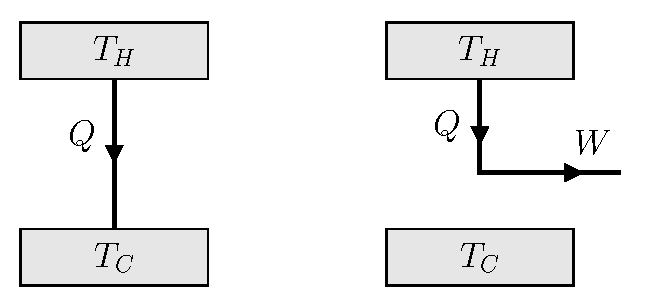
\includegraphics[width=2.7in]{heat_engines/impossible.eps}
\caption{On the left, heat flows from a hot reservoir at temperature $T_H$
  to a cold reservoir at $T_C$.  On the right, how the diagram would
  be altered if we could convert the heat $Q$ into work $W$.}
\label{fig:impossible_engine}
\end{center}
\end{figure}

Can we simply convert all the heat to work?  The first law of
thermodynamics, a.k.a. energy conservation, would have no problem with
this.  This hypothetical engine is illustrated in
Fig.~\ref{fig:impossible_engine}.  In both scenarios in this figure,
the hot reservoir is giving off heat $Q$, and so has negative entropy
change.  Since we are dealing with a reservoir, we use the 
constant temperature approximation (Eq.~\ref{eq:deltaS_isothermal}) to find
\begin{equation}
\Delta S_H = -\frac{|Q|}{T_H}.
\end{equation}
(We use absolute value bars so that there no confusion about the sign
of $Q$).  For the figure on the left, this negative entropy change is
allowed, because it is offset by the positive entropy change of the
cold reservoir, $\Delta S_C=|Q|/T_C$.  But for the figure on the
right, there is no compensating positive entropy change.  And so if we
could convert all heat to work, then
\begin{equation}
\Delta S_\text{total} = \Delta S_H = -\frac{|Q|}{T_H} < 0
\end{equation}
which violates the second law!  So we cannot do this.

But, you may have noticed that we could still satisfy the second law in
the previous example even if we didn't dump all of the heat $Q$ into the
cold reservoir.  Suppose we only dumped enough heat to make the positive
$\Delta S_C$ large enough to compensate for the negative $\Delta S_H$.
That would leave a little energy that we could conceivably convert to
work, while satisfying the second law (and the first, for that matter).

A schematic diagram of this process --- called an {\it engine diagram}
--- is shown in Fig.~\ref{fig:engine_diagram}.  An amount of heat
$Q_H$ is pulled from the hot reservoir, and an amount $Q_C$ is dumped
into the cold reservoir.  In between, some device which we'll call the
working substance intercepts this heat and produces work.  For now,
don't worry about how this might actually be accomplished; we'll
discuss that in detail in the next section.  Instead, focus on the big
picture: such a device will be consistent with the first law as long
as we conserve energy.  Looking at the arrows for energy flow, this
tells us
\begin{equation}
|Q_H| = |Q_C| + |W|. \qquad\text{(first law)}
\end{equation}
Again, we have used absolute value bars everywhere to avoid ambiguity about
whether the symbol $Q_H$ represent the heat flow out of the hot
reservoir (in which case it is a negative value), or the heat flow in
to the work substance (in which case it is positive). 
% To avoid
%confusion, we will use explicit absolute value bars and put the signs
%in ``by hand.''

\begin{figure}
\begin{center}
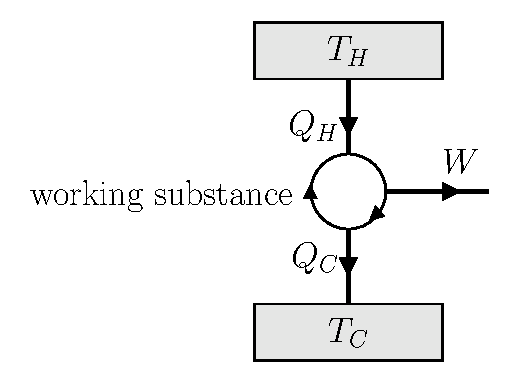
\includegraphics[width=2.4in]{heat_engines/engine_diagram.eps}
\caption{Engine diagram.}
\label{fig:engine_diagram}
\end{center}
\end{figure}

And continuing with the big picture: such a device will be consistent
with the second law as long as the total entropy doesn't decrease.  So
where do entropy changes happen?  Certainly in the reservoirs.  The
hot reservoir has an entropy decrease (since heat leaves the
reservoir) and the cold reservoir has an entropy increase 
(since heat is added to the reservoir).  But what about the 
working substance?  This gets at an
essential point: in order to be a heat engine, the working substance is {\it
  not} a source of energy.  It's not a battery stuck in between the
reservoirs, or anything else consuming chemical energy.  Rather, it
must be returned back to the same state it started from, so the
process can be repeated indefinitely.  But if this is the case, if the
working substance undergoes some cyclic process, then we
can use Eq.~(\ref{eq:DeltaS_cyclic}), which tells us $\Delta
S_\text{w.s.}=0$, since the final and initial states are the same.

And now we can do the complete entropy accounting:
\begin{equation}
  \Delta S_\text{total}= \Delta S_H + \Delta S_C + 
  \cancelto{0}{\Delta S}_\text{w.s.}
  = -\frac{|Q_H|}{T_H}+ \frac{|Q_C|}{T_C}  \geq 0 \quad\text{(second
    law)}
\label{eq:engine_second_law}
\end{equation}

One way to think of Eq.~(\ref{eq:engine_second_law}) is that it gives
a lower bound on how much heat we have to dump to the cold reservoir:
\begin{equation}
|Q_C| \geq \frac{T_C}{T_H}|Q_H|.
\end{equation}
That lower bound isn't zero, so we must dump some heat.
{\it This is an important result\/}:  any heat engine {\it must\/}
dump some of its heat into a cold reservoir.  It is impossible
to turn all heat into usable mechanical energy. 

But the good news is that the lower bound on the dumped heat $|Q_C|$
is smaller than $|Q_H|$, so we do get to ``skim off'' some of the
energy and generate some work.  Notice that the bound on how much heat
we have to dump becomes smaller for very large $T_H$ or small $T_C$.
Evidently, the more extreme the difference in temperature between the
reservoir, the more work we will be able to extract.

Let's quantify that.  Let's introduce a dimensionless quantity called
the efficiency, which is simply the fraction of heat pulled out of the
hot reservoir that we are able to convert to work:
\begin{equation}
\epsilon \equiv \frac{|W|}{|Q_H|}.
\label{eq:efficiency_def}
\end{equation}
From the first law we know $|W|=|Q_H|-|Q_C|$, so we can substitute
this in and write the efficiency equivalently as
\begin{equation}
\epsilon = \frac{|Q_H|-|Q_C|}{|Q_H|} = 1 - \frac{|Q_C|}{|Q_H|}.
\label{eq:general_efficiency}
\end{equation}
Obviously, the efficiency can't ever be greater than 1;
that would correspond to an engine that produces more mechanical energy
than the amount of heat that flows into it, and that would violate the
first law of thermodynamics.  But since $|Q_C|$ can never be zero in
a real engine --- we must always dump some heat --- the efficiency can
never reach 1.   That would violate the second law of thermodynamics.
We'll say more about this in a bit, after we have done a simple example
using efficiency.

\begin{example}{A simple engine problem}
\label{ex:simple_engine}

\begin{figure}[b]
\begin{center}
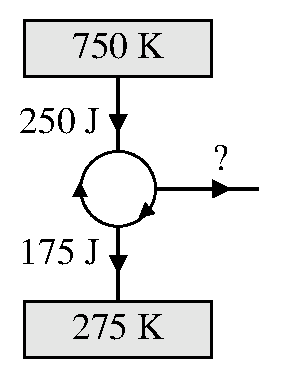
\includegraphics[width=1.1in]{heat_engines/engine_for_example.eps}
\caption{Diagram for Example \ref{ex:simple_engine}}
\label{fig:engine_for_example}
\end{center}
\end{figure}
An engine is described by the engine diagram in
Fig.~\ref{fig:engine_for_example}.  Determine the work output by this
engine and the efficiency of the engine.

\solution
%We could get the answer from Eq.~(\ref{eq:general_efficiency}), but
%we really don't need that. 
We can straightforwardly find the work done
by this engine using the first law of thermodynamics, i.e., energy
conservation.  The energy going into the working substance is
equal to the energy going out of the working substance, so
\begin{equation}
|Q_H| = |Q_C| + |W|
\end{equation}
and
\begin{equation}
|W| = |Q_H| - |Q_C| = 250\units{J} - 175\units{J} = 75\units{J} .
\end{equation}
Then from the definition of efficiency, Eq.~(\ref{eq:efficiency_def}),
we have
\begin{equation*}
\epsilon = \frac{|W|}{|Q_H|}  = \frac{75\units{J}}{250\units{J}} = \boxed{0.30}.
\end{equation*}
\end{example}

Okay, so we have a definition for efficiency, which can never be
greater than one (that would violate the first law of thermodynamics).
But it can never {\bf be equal to} 1 either.\footnote{This is
  important: if you ever calculate an efficiency equal to or greater
  than one, then it is wrong.}  The maximum value of $\epsilon$
corresponds to $|Q_C|$ being at its minimum (since it is being subtracted).
Evidently,
\begin{equation}
\epsilon_\text{max} = 1 - \frac{|Q_{C,{\rm min}}|}{|Q_H|} = 1 -
\frac{(T_C/T_H)|Q_H|}{|Q_H|} = 1-\frac{T_C}{T_H}.
\label{eq:max_efficiency}
\end{equation}
Warning: do not confuse this result for the maximum efficiency
$\epsilon_\text{max}$ with the similar looking expression
Eq.~(\ref{eq:general_efficiency}) for efficiency $\epsilon$ in general.
% Added following in 2010 to keep students from thinking this is
% general
Also, this is only valid if heat is drawn from and dumped into 
isothermal reservoirs.

It is worth keeping in mind that Eq.~(\ref{eq:max_efficiency}) for the
maximum efficiency is really a special case of an engine operating
between two thermal reservoirs.  A more general approach is just to
use the first and second laws of thermodynamics.  The first law just says
balance the energy in and the energy out, and the second law says
% In fact, using the
%first and second laws is preferable, because
%Eq.~(\ref{eq:max_efficiency}) only works if the engine operates
%between two thermal reservoirs.  This approach 
%
%will work for both
%simple reservoir problems and more complicated problems as well.
\begin{equation}
\Delta S_\text{total} = 0 \qquad\text{(maximum efficiency)}
\end{equation}
Ultimately, that's the one equation you need to remember
to solve problems involving a maximally efficient engine.

Let's consider some examples:
\newpage

\begin{example}{Automobile Efficiency}

\label{example:automobile_efficiency}

The internal combustion engine of an automobile is a heat engine.
Yes, there is gas being consumed, but that's being burned to provide
the high temperature of the hot reservoir.  From there on, the engine
functions as a heat engine.  

The hot reservoir is about $820^\circ\units{C}$ and the cold reservoir
is almost air temperature, but typically more like
$70^\circ\units{C}$.  Burning a gallon of gasoline provides about
$120\units{MJ}$ of heat.  What is the upper limit on how much work can
be extracted from a gallon of gas, and how much heat must be dumped?

\solution The moment you see the words ``upper limit'' (or similar
language), then you can pull out the second law of thermodynamics:
$\Delta S_\text{total} = 0$.  For this problem, $\Delta S_\text{total}
= \Delta S_H + \Delta S_C$, since the reservoirs are the
only parts of this system whose entropy changes.

To calculate $\Delta S$ for the reservoirs, we need to convert the
temperatures to Kelvin, so $T_H=820+273=1093\units{K}$ and
$T_C=70+273=343\units{K}$.  The entropy change of the hot reservoir is
\begin{equation}
\Delta S_H = \frac{-|Q_H|}{T_H} = 
-\frac{120\times 10^6\units{J}}{1093\units{K}}
 = -1.10\times 10^{5}\units{J/K}
\end{equation}
Therefore, since $\Delta S_\text{total} = 0$, it follows that  
$\Delta S_C$ must be positive by at least this amount.
\begin{equation}
\Delta S_{C,{\rm min}} = \frac{|Q_{C,{\rm min}}|}{T_C} = 1.10\times
10^5\units{J/K}
\end{equation}
so
\begin{equation}
|Q_{C,{\rm min}}| = 343\units{K} \cdot 1.10\times 10^{5}\units{J/K} =
\boxed{37.7\units{MJ}.}
\end{equation}
We get the maximum work by subtracting this from $|Q_H|$:
\begin{equation}
|W_\text{max}| = 120 - 37.7 = \boxed{82\units{MJ}.}
\end{equation}
In reality, the work output is only about 1/3 of this amount, due to
(i) design choices to get the work out faster, i.e. to get more power,
(ii) friction, and (iii) imperfect combustion of the fuel.
\end{example}

We could have solved the previous example by using the equation for
$\epsilon_\text{max}$ for engines with thermal reservoirs (although 
there was no need to do so).  The following is an example where 
the $\epsilon_\text{max}$ approach would not work; i.e., you
{\bf must} start from the second law of thermodynamics:
\begin{example}{A Two-Brick Heat Engine}
  \label{example:two_brick_heat_engine}
  A hot brick initially at temperature $T_H=400\units{K}$ is used as
  the source for a heat engine.  An equal sized cold brick made of the
  same material, initially at temperature $T_C=300\units{K}$, is used
  to dump the waste heat.  As the heat flows, the two bricks come to
  thermal equilibrium.  Assuming the heat engine was maximally
  efficient, what is the final temperature?

  \solution You might think the final temperature should just be
  $350\units{K}$, but that would be true only if we didn't intercept
  any of the heat and convert it to work.

  There is a lot we aren't given.  We don't know the amounts
  or the composition of the bricks, but we know they are identical.
  The hotter brick is going to cool from $400\units{K}$ down to some
  $T_f$, so its entropy change will be $\Delta S_H = nC\ln(T_f/400)$,
  which is negative since $T_f/400<1$.  The colder brick will warm
  from $300\units{K}$ to $T_f$, so its entropy change will be $\Delta
  S_C=nC\ln(T_f/300)$.  For maximum efficiency, then,
\begin{equation}
\Delta S_\text{total} = \Delta S_H+ \Delta S_C =
nC\ln\left(\frac{T_f}{400}\right) + nC\ln\left(\frac{T_f}{300}\right)
= 0.
\end{equation}
The $nC$ factors divide out, and we get
\begin{equation}
  \ln T_f - \ln 400 + \ln T_f - \ln 300 = 0
%\ln\left(\frac{T_f}{400}\right) =-\ln\left(\frac{T_f}{300}\right)
% = \ln\left(\frac{300}{T_f}\right)
\end{equation}
and so
\begin{eqnarray}
2\ln T_f = \ln(400\cdot 300) \quad&\Rightarrow&\quad 
%\frac{T_f}{400}= \frac{300}{T_f} \quad\Rightarrow\quad
T_f^2=400\cdot 300  \nonumber \\ 
      &\Rightarrow&\quad \boxed{T_f = 346.4\units{K}.} 
\end{eqnarray}
We see that the bricks end up slightly cooler than $350\units{K}$,
which makes sense since we skimmed off some of the energy as it was
flowing from hot to cold.
\end{example}

\section{Gas Cycles for Heat Engines}

We have made the case that skimming off some heat flow and generating
work is possible, that is, consistent with energy conservation and the
second law.  But how do we actually make a heat engine?  We need to
find some working substance that can take in heat, do work, and dump
heat.  We do not have to look very far: an ideal gas will do the job
nicely.  In fact, gases are the most commonly used substance in heat
engines today.

Consider a gas enclosed in a cylinder with a movable piston, as shown
in Fig.~\ref{fig:gas_piston}.  Recall that the work done by a gas is
given by
\begin{equation}
W_\text{by} = \int_A^B p\,dV,
\end{equation}  
so the gas can do work if we let the piston expand.  We can put heat
into the gas by bringing it into contact with something at a higher
temperature, and we can dump heat out of the gas by bringing it into
contact with something at a lower temperature.  To be useful, we will
want to complete a full cycle, to bring the gas back to its starting
point.  This means contracting the piston at some point in the cycle,
which will cost work (i.e., work is done {\bf on} the piston, or
work done {\bf by} the piston is negative).   But part of the cycle
will involve an expansion, and that produces positive work by the
piston.  Overall, we can get work out of the process (i.e., the net 
work by the piston is positive) if the expansion
happens with higher pressure (so more force) than the contraction.

A typical cycle is illustrated in Fig.~\ref{fig:gas_piston}. Notice
that the expansion happens at higher pressure than the compression,
leading to a net work being done by the gas.  These gas cylinders are
often paired up, as in an automobile, so that the expansion of one
cylinder causes the compression of the other cylinder, with power left
to spare.

\begin{figure}
\begin{center}
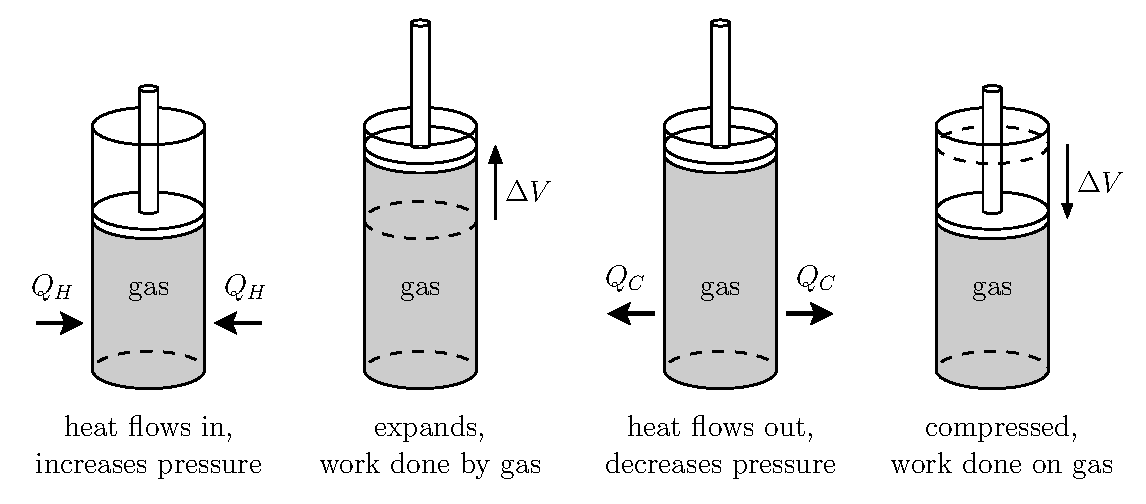
\includegraphics[width=5.5in]{heat_engines/gas_piston.eps}
\caption{Caption for gas-piston figure}
\label{fig:gas_piston}
\end{center}
\end{figure}

To quantify the cyclic gas process, it is useful to plot it on a
$p$\,-$V$ diagram.  One such cyclic process is illustrated in
Fig.~\ref{fig:rectangle_cycle}, which is a sequence of constant
pressure and constant volume processes that leads to a rectangular
cycle on the $p$\,-$V$ diagram.  Let's analyze this case in some detail,
starting with a calculation of the net work for the whole cycle.

\begin{figure}
\begin{center}
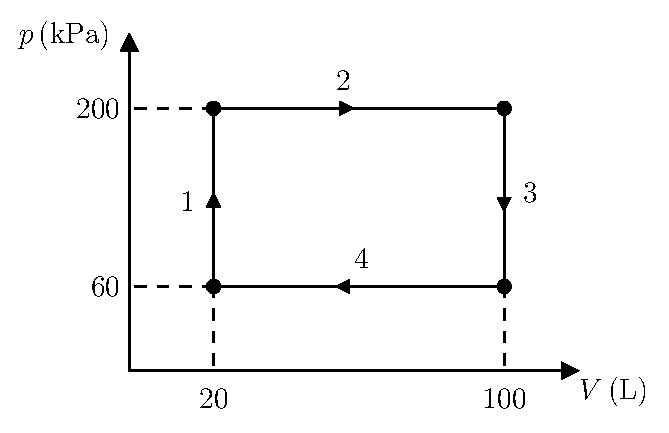
\includegraphics[width=3in]{heat_engines/rectangle.eps}
\caption{Cyclic process made up of constant pressure and constant volume
processes.}
\label{fig:rectangle_cycle}
\end{center}
\end{figure}

The constant volume steps do no work, while for constant pressure,
$W_\text{by}=p\Delta V$.  Adding this up around the whole cycle gives
\begin{align}
W_\text{cycle} &= W_1 +  W_2 + W_3 + W_4 \nonumber\\
 &= 0 + 200 \units{kPa}(+80\units{L}) + 0 +
 60\units{kPa}(-80\units{L})  = 140\cdot 80 \units{kPa$\cdot$L}\nonumber\\
&= 11.2\units{kJ}
\label{eq:work_for_rectangle}
\end{align}
Notice that the work done in the cycle is just the area of the enclosed
rectangle, which is true for any cycle.

Now let's figure out what $|Q_H|$ and $|Q_C|$ are.  For this we will
need to know whether the gas is monatomic or diatomic.  Let's assume
the gas is diatomic, so $f=5$ and $\gamma=1.4$.  For the constant
volume processes (steps 1 and 3 in Fig.~\ref{fig:rectangle_cycle})
there is no work done by the gas, so the first law says
\begin{equation}
 Q = \Delta E_\text{therm}+ 0 = {\textstyle\frac{5}{2}} \Delta(pV)
 = \textstyle{\frac{5}{2}} V\Delta p,
\end{equation}
where we've used the fact that $V$ is a constant in the last step.
Now we can calculate the heat flow into the gas for steps 1 and 3:
\begin{align}
Q_1 &= {\textstyle\frac{5}{2}}\cdot  20\units{L}\cdot (200\units{kPa}-60\units{kPa}) =
7.0\units{kJ}\nonumber\\
Q_3 &= {\textstyle\frac{5}{2}}\cdot  100\units{L} \cdot (60\units{kPa}-200\units{kPa}) =
-35.0\units{kJ}.
\end{align}
For a constant pressure process (steps 2 and 4 in
Fig.~\ref{fig:rectangle_cycle}) the work is $p\, \Delta V$ and so the
first law says
\begin{equation}
Q = \Delta E_\text{therm}+ W_\text{by} = {\textstyle\frac{5}{2}}\cdot \Delta(pV) +
p\Delta V = {\textstyle\frac{7}{2}}\cdot  p\Delta V.
\end{equation}
where we've used the fact that $p$ is a constant in the last step.
Now we can compute
\begin{align}
Q_2 &= {\textstyle\frac{7}{2}}\cdot  200\units{kPa}\cdot (100\units{L} - 20\units{L})
 = 56.0\units{kJ} \nonumber\\
Q_4 &= {\textstyle\frac{7}{2}}\cdot 60\units{kPa}\cdot (20\units{L} - 100\units{L})
 = -16.8\units{kJ} 
\end{align}
We have calculated the heat flow into the gas for each step.  Now we
can identify $Q_H$ as coming from all the steps with positive $Q$,
where heat really does flow in.  In our example, this would be steps 1
and 2.  In contrast, $Q_C$ comes from all the steps with negative $Q$,
where heat is actually flowing out of the gas, which is steps 3 and 4
for our example.  So we can calculate
\begin{align}
|Q_H| &= Q_1 + Q_2 = 7 + 56 = 63.0\units{kJ} \nonumber\\
|Q_C| &= |Q_3| + |Q_4| = 35 + 16.8 = 51.8\units{kJ}.
\end{align}
We can check our calculation, since we have already computed the work
in Eq.~(\ref{eq:work_for_rectangle}):
\begin{equation}
|W| = |Q_H|-|Q_C| = 63.0 - 51.8 = 11.2\units{kJ} \quad \surd
\end{equation}
And finally we can compute the efficiency,
\begin{equation}
\epsilon = \frac{|W|}{|Q_H|} = \frac{11.2}{63.0} = 0.178.
\end{equation}

This rectangular gas cycle engine is not actually practical.  Automobiles
use instead something called the Otto cycle, which is a sequence of
constant volume and adiabatic processes, as illustrated in
Fig.~\ref{fig:otto_cycle}.

\begin{figure}
\begin{center}
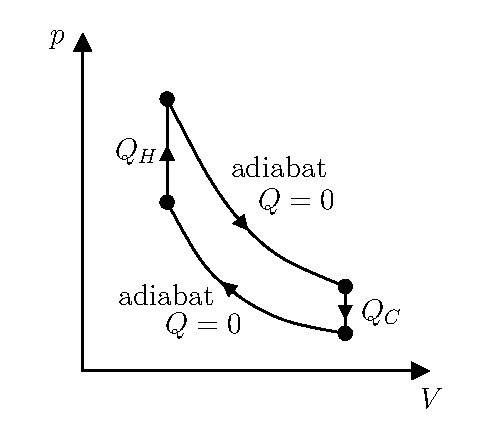
\includegraphics[width=2.5in]{heat_engines/otto_cycle.eps}
\caption{Otto cycle.}
\label{fig:otto_cycle}
\end{center}
\end{figure}

The heat for the constant volume steps is again given by
\begin{equation}
Q = \Delta E_\text{therm} = \frac{f}{2}V\Delta p \qquad\text{(constant
  volume)}
\end{equation}
which is positive when the pressure increases and negative when it
decreases.  And now for the nice part: by definition there is no heat flow during
either of the adiabatic steps, so these constant volume processes give
$Q_H$ and $Q_C$ as labeled in Fig.\ref{fig:otto_cycle}.  In the
homework problems you will work out the details of the Otto cycle.

The adiabats are exactly what makes this a more practical engine.
The adiabatic expansion and compression steps happen very quickly,
which is why no heat flows because it simply doesn't have enough time
to flow.  But this means a cycle is completed relatively quickly, and
so we are getting the work of the cycle out in a short amount of
time.  Recalling that work per time is power, we see that having a
fast cycle can lead to more power output, which is often desired.

\section{Refrigerators}

An interesting thing happens if we take a heat engine and run it
backwards: we make a refrigerator.  By refrigerator, we mean a device
which requires work as input and is able to make heat flow from a
colder object to a hotter object.  This includes, of course, the
refrigerator that keeps your milk from getting spoiled, but also
includes air conditioners and even heat pumps (which is basically an
air conditioner hooked up backwards to cool the outdoors and warm
your house).

Making heat flow from cold to hot may sound like a violation of
Clausius's statement of the second law, but it is not as long as
something else is going on in the process.  Heat will not
{\it spontaneously\/} flow from cold to hot; rather, we must cleverly
engineer the refrigerator to make it happen and, most importantly, we
must plug it in, to give the necessary work as input.

\begin{figure}
\begin{center}
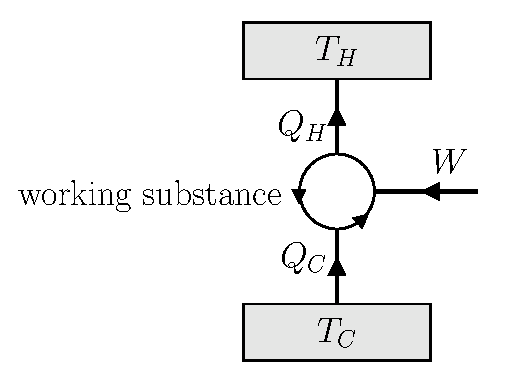
\includegraphics[width=2in]{heat_engines/refrigerator_diagram.eps}
\caption{A refrigerator diagram, made by reversing all the arrows on a
  heat engine diagram.  Note that the working substance cycle is now
  counterclockwise instead of clockwise.}
\label{fig:refrigerator_diagram}
\end{center}
\end{figure}

Let's start with an engine diagram in reverse, as shown in
Fig.~\ref{fig:refrigerator_diagram}, and focus on the first and second
laws.  Energy conservation now requires
\begin{equation}
|Q_C| + |W| = |Q_H| \qquad\qquad\text{(first law)}
\end{equation}
which is exactly the same equation as before, since we reversed {\it
  all\/} the arrows.  Now the signs of the entropy change in the
reservoir are reversed, so the second law says
\begin{equation}
\Delta S_\text{total} = \Delta S_H + \Delta S_C = 
 \frac{|Q_H|}{T_H} - \frac{|Q_C|}{T_C} \geq 0.\quad\text{(second law)}
\end{equation}
 This now provides an {\it upper\/} bound on $|Q_C|$, namely
\begin{equation}
|Q_C| \leq \frac{T_C}{T_H}|Q_H|.
\label{eq:qc_upper_bound}
\end{equation}

What does this mean?  It means we can run a heat engine backwards and
satisfy the first and second laws and actually make some heat go from
cold to hot.  But there is a limitation on how much heat we can pull
out of the cold reservoir, and this limitation depends on the
reservoir temperatures and on how much work we provide.  If we
eliminate $|Q_H|$ from the upper bound, Eq.~(\ref{eq:qc_upper_bound}),
we can show
\begin{equation}
|Q_C| \leq \frac{T_C}{T_H-T_C} |W|,
\label{eq:qc_upper_bound_ii}
\end{equation}
which you will derive in the homework.  This expression says that we
need work to pull heat out of the cold reservoir, and also that the
effectiveness of pulling out heat will depend on the reservoir
temperatures.  We can quantify this ``effectiveness'' with what is
called the coefficient of performance, $CP$, defined as the ratio of
what want ($|Q_C|$) to what we must pay ($|W|$):
\begin{equation}
CP = \frac{|Q_C|}{|W|} \leq  \frac{T_C}{T_H-T_C}.
\end{equation}
As before, the maximum coefficient of performance is obtained from the
borderline case of the second law $\Delta S_\text{total}=0$.
Notice that reservoirs that are close in temperature yield a larger
$CP$.  This makes sense, since the closer $T_H$ and $T_C$ are, the
less ``uphill'' we are making the heat flow.

In the refrigerator diagram the working substance now goes
through a counterclockwise gas cycle.  This allows for the heat to
flow into the gas while it is at a lower temperature (lower than
$T_C$) and heat to flow out of the gas while it is at a higher
temperature (higher than $T_H$).  But this counterclockwise cycle also
means compression happens at higher pressure than the expansion.  This
will require some outside source of work to drive the gas through this
cycle, which is exactly what we found from general first law and
second law considerations: work input is necessary to make the
refrigerator function.  In other words, your refrigerator won't function
properly if you forget to plug it in.



\newpage

\section*{Problems}
\markright{PROBLEMS}

\begin{problem} 
  A $36\units{g}$ ice cube at $0^\circ\units{C}$ is dropped into
  $90\units{g}$ of water at $22^\circ\units{C}$.  Heat flows from the
  water to the ice, bringing both to equilibrium at
  $0^\circ\units{C}$.
  \begin{enumerate}
  \item Determine the number of moles of ice melted in cooling the
    water to $0^\circ\units{C}$.
  \item Calculate the entropy change of the melted ice.
  \item Calculate the entropy change of the $90\units{g}$ of water 
   in this process.  Is your answer consistent
    with the second law?
  \end{enumerate}
\label{prob:iceintowater}
\end{problem}

\begin{problem}
  Consider a pair of $5.0\units{mol}$ ideal solids.  Solid $A$ initially has
  a temperature of $500\units{K}$, while solid $B$ has a temperature of
  $200\units{K}$.  The solids are brought into thermal contact, and
% Added in 2010.
  heat flows until the system reaches equilibrium.
  Determine the entropy change of each solid, and the total entropy
  change. 
\end{problem}

\begin{problem}
  By what factor is the multiplicity increased in melting
  $18\units{g}$ of $0^\circ\units{C}$ ice into $0^\circ\units{C}$ water?
\label{prob:multiplicityformelting}
\end{problem}

\begin{problem} 
% an assigned problem to make the point that eps \neq eps_max
  A heat engine draws $600\units{J}$ of heat per cycle from a hot
  reservoir at $800\units{K}$, and dumps $300\units{J}$ of heat per
  cycle into a cold reservoir at $200\units{K}$.  Determine the
  efficiency of this engine.
\label{prob:simpleengine}
\end{problem}

\begin{problem}
  Consider a $10\units{mol}$  brick of ideal solid initially at temperature
  $500\units{K}$.  This brick is used as the heat source for a heat
  engine, which is dumping heat to a room-temperature reservoir at
  $295\units{K}$.
  \begin{enumerate}
  \item Determine the entropy change of the brick as it cools to room
    temperature.
  \item Determine the minimum amount of heat that must be dumped by
    this heat engine.
  \item Calculate the efficiency of this best-case engine.
  \end{enumerate}
\label{prob:onebrickengine}
\end{problem}

\begin{problem} 
  Consider the two-brick heat engine of
  Example~\ref{example:two_brick_heat_engine}.  Calculate the maximum
  amount of work that could be obtained from this engine.  For this
  problem, assume that the bricks are each an ideal solid with 
  $2.0\units{mol}$.  
\label{prob:twobrickengine}
\end{problem}
\newpage

\begin{problem} 
  Susquehanna Valley Limousine has modified their automobile engine to
  provide heat for an oven to bake fresh chocolate chip cookies while
  you cruise Lewisburg.\footnote{Not really.}  For each gallon of gas,
  $12\units{MJ}$ of heat is dumped from the engine into the oven at a 
  temperature of $190^\circ\units{C}$, and the remainder of the heat 
  coming from the engine is dumped to the environment at 
  $70^\circ\units{C}$, as described in 
  Example~\ref{example:automobile_efficiency}.  Calculate the maximum
  work possible from a gallon of gas for this engine.  As in 
  Example~\ref{example:automobile_efficiency}, assume that the hot
  reservoir has a temperature of $820^{\circ}\units{C}$ and the 
  heat coming from the burning gas totals $120\units{MJ}$.
  \begin{figure}[h]
   \begin{center}
   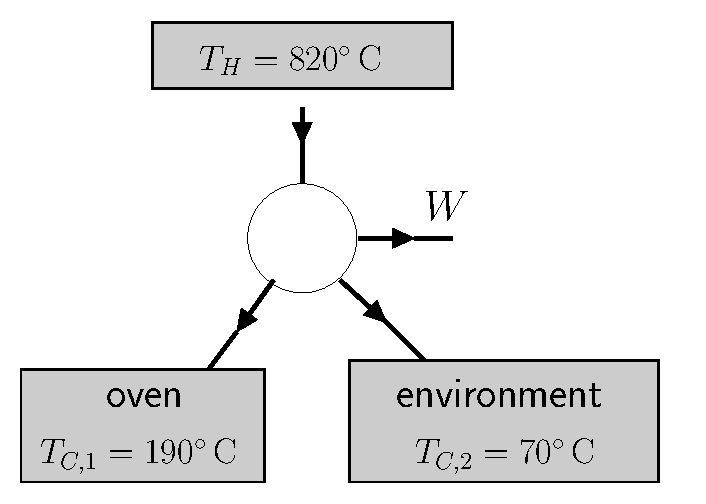
\includegraphics[width=3.0in]{heat_engines/limousine.eps} 
   \end{center} 
   \caption{Engine diagram for Problem \ref{prob:limousine}}
   \end{figure}
\label{prob:limousine} 
\end{problem}
\newpage

\begin{problem}  % A55, brought into chapter
  In the cycle shown below, $1.0\units{mol}$  of a
  monatomic ideal gas is initially at a pressure of $p_A=100\units{kPa}$
  and a temperature of $T_A=0^\circ\units{C}$.  The gas is heated at
  constant volume to $T_B = 150^\circ\units{C}$ and is then expanded
  adiabatically until its pressure is back to $p_C=100\units{kPa}$.
  Finally, the gas is compressed at constant pressure until it is back
  to its original state $A$.  Find
  \begin{enumerate}
  \item the pressure, volume and temperature for each of the three
  labeled points (A, B and C),
  \item the heat entering or leaving the system during each process, and
  \item the efficiency of this cycle.
  \end{enumerate}
  \begin{figure}[h]
    \begin{center}
      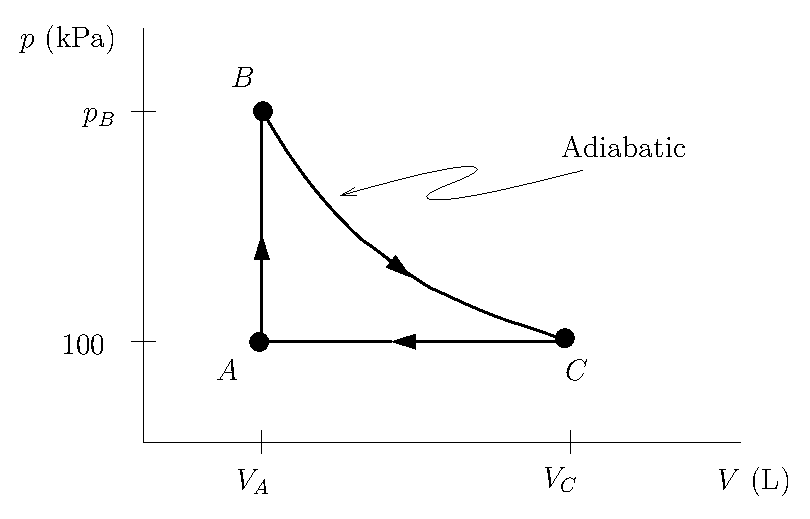
\includegraphics[width=3.5in]{heat_engines/cycle.eps}
    \end{center}
    \caption{Cycle for Problem \ref{prob:threelegcycle}} 
  \end{figure}
\label{prob:threelegcycle}
\end{problem}

\begin{problem} 
  For the rectangular gas cycle in Fig.~\ref{fig:rectangle_cycle},
  assume that there is $0.50\units{mol}$ of diatomic gas.
  \begin{enumerate}
  \item If this cycle is to operate between two reservoirs, calculate
    the minimum possible value for $T_H$ and the maximum value for
    $T_C$.
  \item Compare the efficiency of this gas cycle to the maximum
    efficiency possible for a cycle operating between these two
    reservoirs.
  \end{enumerate}
\label{prob:rectangularcycle}
\end{problem}

\begin{problem} 
  Explain why, for any gas cycle that is clockwise on a $p$\,-$V$
  diagram, the area enclosed by the loop gives the net work by the gas
  in the cycle.
\end{problem}

\begin{problem} 
  Is an automobile engine more efficient in the summer or the 
  winter?
  Explain using general entropy/heat engine arguments, and also with a
  $p$\,-$V$ diagram. (Note:  overall gas mileage for a car also depends
  quite strongly on tire pressure, which can also vary between the summer
  and winter.)  Assume that the temperature to which the hot gasoline vapors
are raised during  combustion  is unchanged.
\end{problem}

\begin{problem} 
  An Otto cycle for a fixed number of moles of a diatomic ideal gas is shown in
  Fig.~\ref{fig:otto_cycle_hw}. 
  \begin{figure}[h]
    \begin{center}
      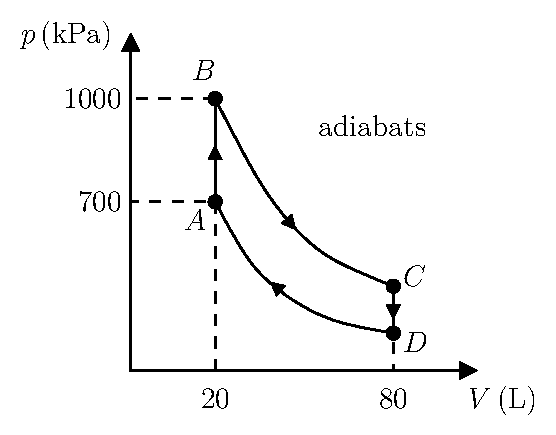
\includegraphics[width=3in]{heat_engines/otto_cycle_hw.eps}
      \caption{Otto cycle for Problem~\ref{prob:otto_cycle}.}
      \label{fig:otto_cycle_hw}
    \end{center}
  \end{figure}
   \begin{enumerate}
   \item Calculate the pressure at points $C$ and $D$.
   \item Determine $|Q_C|$, $|Q_H|$, and $|W|$ for one cycle.  {\it
       Hint:} save $|W|$ for last.
   \item Calculate efficiency of this cycle. 
   \end{enumerate}
   \label{prob:otto_cycle}
\end{problem}

% \begin{problem} {\bf Maximally efficient engine.} [in development]
%  Consider the following gas cycle: (i) isothermal expansion at
%  temperature $T_H$, (ii) adiabatic expansion until the gas cools to
%  $T_C$, (iii) isothermal compression at temperature $T_C$, and (iv)
%  adiabatic compression until the gas temperature reaches $T_H$.
%  Calculate $\epsilon$, compare to $\epsilon_\text{max}$.  Called
%  Carnot engine.  (b) why is this ideal?  Isotherms: heat flow between
%  (nearly) identical temperature reservoir and gas, (nearly) zero
%  entropy produced.  Adiabats: no heat flow, no entropy change.  Needs
%  work.
% \end{problem}

\begin{problem} 
  Derive Eq.~(\ref{eq:qc_upper_bound_ii}), the upper bound for $|Q_C|$
  in a refrigerator, by starting from the first and second laws.
\end{problem}

\begin{problem}
  Can you cool off your house by opening the door to the refrigerator?
  Explain why or why not.
\end{problem}


\begin{problem} 
 A  refrigerator is designed to  keep its interior  at a constant
  $5^\circ\units{C}$  while  dumping  heat  into  a  room  temperature
  environment at $22^\circ\units{C}$.  The interior of
  the refrigerator may be regarded as a cold reservoir, 
while the air  around it is a
  hot reservoir.  Now suppose  a pitcher containing $1800\units{g}$ of
  room-temperature water  is put into  the refrigerator. We  can break
  down what happens next into two  steps: (1) the water will cool down
  to the  temperature of the  cold reservoir (fridge interior)  as its
  heat flows into  cold reservoir, and (2) the  refrigerator will turn
  on and do  work (run a compressor, circulate  refrigerant, etc.)  to
  extract this  heat from  the cold  interior and dump  it to  the air
  outside.

We'll calculate what happens in each of these steps.

Step \#1:
\begin{enumerate}
\item  Calculate the change in entropy of the water as it cools from 
$22^\circ\units{C}$ to $5^\circ\units{C}$.
\item Calculate the change in entropy of the cold reservoir (i.e. the
inside of the refrigerator) due to this same heat transfer.

\item Is the second law of thermodynamics satisfied in this step?
Explain briefly why or why not, using your results above.
\end{enumerate}

Step \#2
\begin{enumerate}

\item Now we must get rid of the extra heat in the cold reservoir 
  by   transferring  it  to  the  hot  reservoir.
  Calculate the change in the entropy of the cold reservoir
(refrigerator) as the excess heat
  from step \#1 is removed from the refrigerator's interior.

\item  Determine the minimum amount  of work required to remove this 
excess heat
from the cold reservoir. 

% \item  Optional: Is this two-step refrigerator maximally efficient in cooling
% the water?  If so, how do you know? If not, can you think of a way to make it more efficient?

\end{enumerate}
\end{problem}


% \begin{problem} 
%   A refrigerator is designed to dump heat into a room temperature
%   environment at $22^\circ\units{C}$ while keeping the interior at  
%   $5^\circ\units{C}$.   In this problem, you may treat the interior 
%   of the refrigerator as a cold reservoir.  If you put pitcher containing
%   $1800\units{g}$ of room temperature water into to the refrigerator, it 
%   will cool down to the temperature of the interior reservoir, dumping 
%   heat into the cold reservoir.  What is the minimum amount of work 
%   required to remove this heat from the interior of the refrigerator.
% \end{problem}

% \begin{problem} 
%  Hard (do we want this?): rectangle pV diagram: why can't this be a
%  refrigerator?  Hint: think about where on the cycle $Q_h$ and $Q_C$
%  occurs, and what the temperature of the working substance (the gas)
%  is at that point in the pV diagram.  Is there any similar
%  restriction on heat engines?  I.e. some pV cycles that can't be heat
%  engines?
% \end{problem}
